\documentclass{beamer}

\usepackage[utf8]{inputenc}
\usepackage[ngerman]{babel}
\usepackage{beamerthemeshadow}
\usepackage{calc}
\usepackage{ifthen}
\usepackage{tikz}
\usepackage{caption}
\usepackage{subcaption}
\usepackage{bchart}
\usepackage{wrapfig}
\usepackage{ulem}
\usepackage{color}
\usepackage{epigraph}
\usepackage{tipa}
\usepackage{hyperref}
\usepackage{url}
\usepackage{amsmath}

\usepackage[
	european,
	europeanvoltages,
	europeanresistors,
	europeanports
]{circuitikz}

% \usepackage{pgf-pie}

\definecolor{darkgreen}{rgb}{0.2,0.6,0.2}

\usepackage{listings}

\title{Dimensionierung einer AC-Verstärkerschaltung}
\subtitle{ET+ELO Labor, Teil 1}
\author{E. Mazlagi\'c, M. Müller}
\institute{Hochschule Luzern \\ Technik \& Architektur}


% Listing settings
% \lstset{
%    %breakwhitespace=true,
%    language=[LaTeX]TeX,
%    basicstyle=\footnotesize\ttfamily,
%    keywordstyle=\color{red}\bfseries,
%    idnetifierstyle=\color{blue},
%    commentstyle=\color{darkgreen},
%    stringstyle=\color{blue},
%    columns=fullflexible,
%    keepspaces=true,
%    breaklines=true,
%    tabsize=3,
%    showstringspaces=false,
%    extendedchars=truei
%    morekeywords={
%	\begin, 
%	\item,
%	\end}
%}


\begin{document}
\maketitle

\section{Aufgabenstellung}

\subsection{Schaltung}

\begin{frame}
	\frametitle{Schaltung}
	\begin{figure}
		\centering
		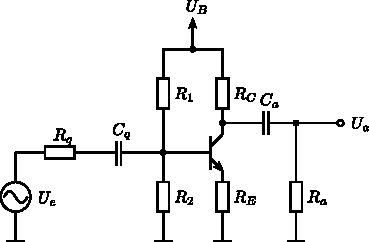
\includegraphics[scale=1.2]{ac-amp.pdf}
		\caption{AC-Verstärkerschaltung}
	\end{figure}
\end{frame}

\section{Dimensionierungen}

\subsection{Widerstände}

\begin{frame}
	\frametitle{Ausgangsseite}
		\begin{block}{Richtwert für $R_C$}
			Der Richtwert gibt an, dass
			\[R_C < 0.3 \cdot R_L \]
			gelten muss.
		\end{block}
			$\Rightarrow R_C = 0.3 \cdot 22k \Omega = 6.6k \Omega$
			$\xrightarrow{E12} 5.6k \Omega$

		\[ R_E = \frac{\beta \cdot R_C - V_U \cdot R_{BE}}
		{V_U \cdot (1+\beta)} \approx \frac{R_C}{V_U} =
		\frac{5.6k \Omega}{5.62} = 
		996.4 \Omega \xrightarrow{E12} 1k \Omega \]
\end{frame}

\begin{frame}
	\frametitle{Ausgangsseite}
		\begin{block}{Regel für $\frac{R_C}{R_E}$}
			Die Regel besagt, dass 
			\[ \frac{R_C}{R_E} < 10 \]
			sein muss. Ist dies nicht gegeben, so muss zum
			Emitterwiderstand ein RC-Glied parallel geschaltet
			werden.	
		\end{block}
				
\end{frame}

\section{Messung}

\subsection{Erste Messung}

\begin{frame}
	\frametitle{Erste Messungen}
	\begin{block}{Parameter}
	$U_{qpp} = 2V$, $U_B = 20V$
	\end{block}

	\begin{block}{Ausgangsignal}
	$U_{a_{pp}} = 8.1V$, $U_{RE_{pp}} = 1.85V$, $U_{R_{2_{pp}}} = 1.92V$,
	$A_V = 12.15dB$
	\end{block}

	\begin{alertblock}{Konsequenz}
	Ein grösserer Basisstrom ist nötig $\rightarrow R_1$ kleiner oder 
	$R_2$ grösser wählen.
	\end{alertblock}	
	
\end{frame}

\begin{frame}
	\begin{figure}
		\centering
		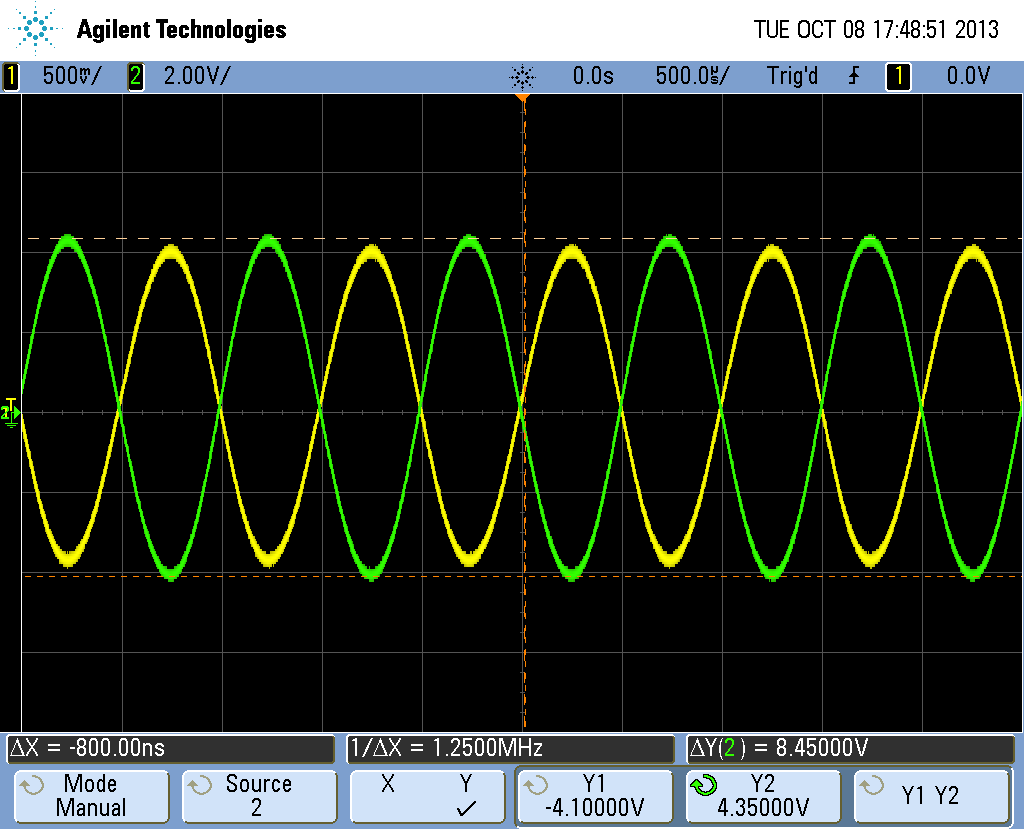
\includegraphics[width=0.7\textwidth]{scope_0.png}
		\caption{$U_a$ vs. $U_e$}
	\end{figure}
\end{frame}

\begin{frame}
	\begin{figure}
		\centering
		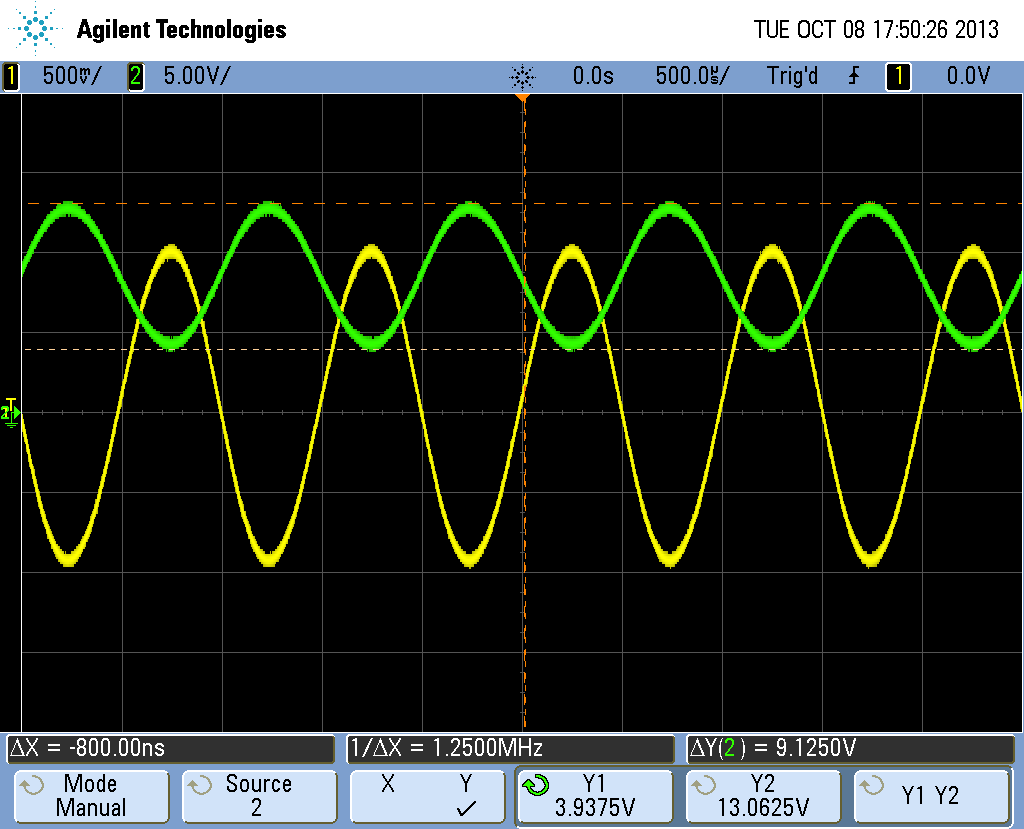
\includegraphics[width=0.7\textwidth]{scope_1.png}
		\caption{$U_C$ vs. $U_e$}
	\end{figure}
\end{frame}

\begin{frame}
	\begin{figure}
		\centering
		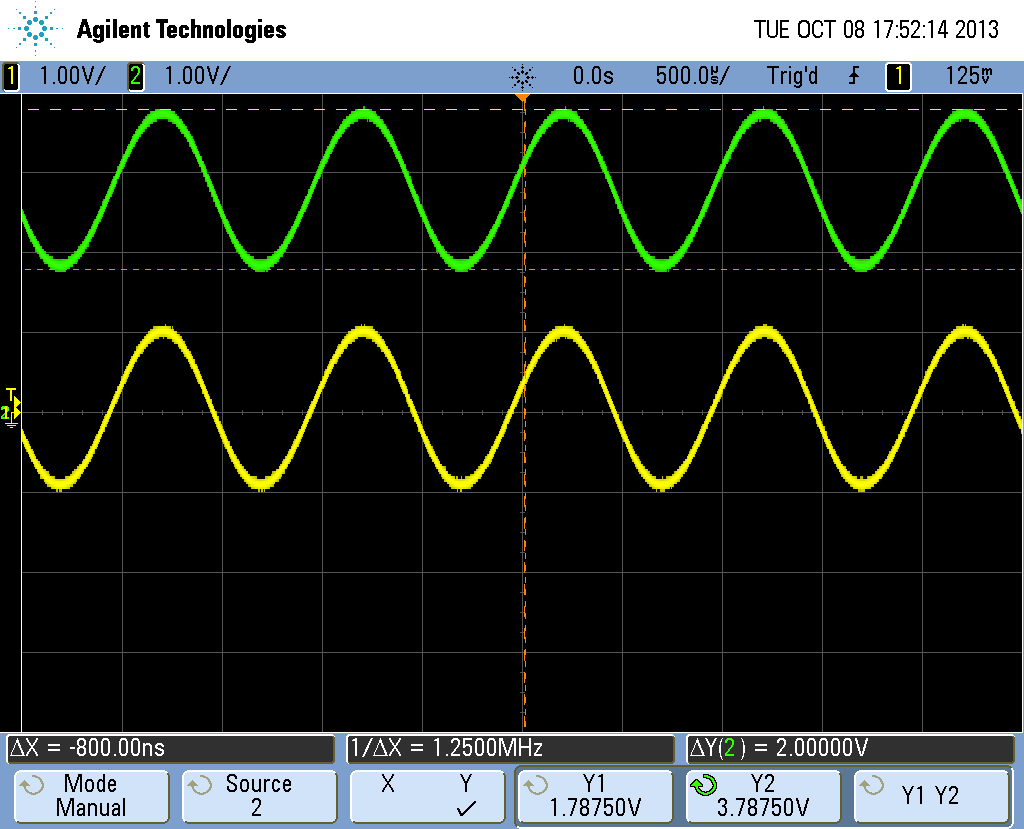
\includegraphics[width=0.7\textwidth]{scope_2.png}
		\caption{$U_{R_2}$ vs. $U_e$}
	\end{figure}
\end{frame}

\begin{frame}
	\begin{figure}
		\centering
		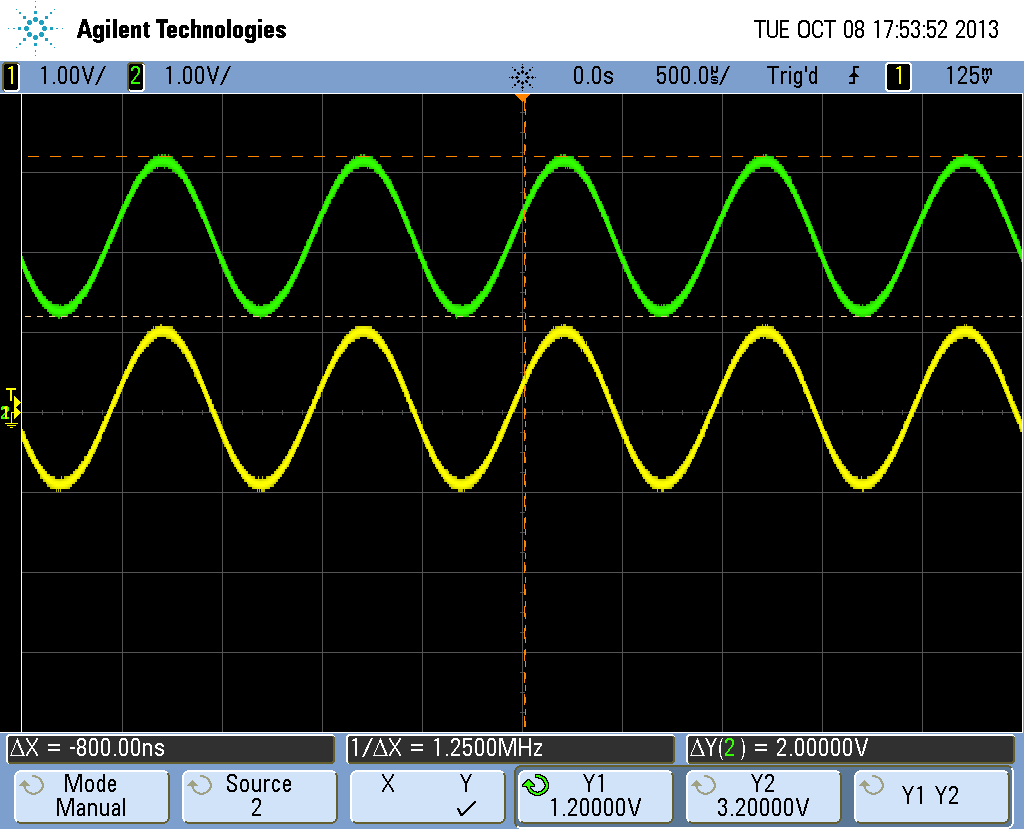
\includegraphics[width=0.7\textwidth]{scope_3.png}
		\caption{$U_{R_E}$ vs. $U_E$}
	\end{figure}
\end{frame}

\begin{frame}
	\frametitle{Anpassungen}
	\begin{enumerate}
		\item Verstärkung zu klein $\Rightarrow R_1$ verkleinern 
		\item Aussteuerungsgrenze erreicht $\Rightarrow R_2$ vergrössern
		\item Arbeitspunkt zu tief $\Rightarrow R_C$ verkleinern
	\end{enumerate}
	Mit diesen Anpassungen haben wir folgende Werte erreicht:
	\begin{itemize}
		\item $U_{q_{pp_{max}}} = 0.8V$
		\item $U_A = 3V$
		\item $A_V = 11.48dB$
	\end{itemize}
	Um den optimalen AC-Verstärker zu erstellen, müssten alle Widerstände
	aufeinander angepasst werden.
\end{frame}


\end{document}
